\begin{slikaDesno}{fig/cconv_setup.pdf}
\PID \label{z:kruz_konv}
За периодичне сигнале са основним 
периодом $T$ може се дефинисати 
операција \textit{периодичне
конволуције} као 
$$x \circledast y = \int_{t_0}^{t_0 + T} 
x(\uptau) y(t-\uptau) \, \de \uptau,$$
где је $t_0$ произвољна константа. Периодична поворка  униполарних
правоугаоних импулса једнаког трајања импулса и паузе,
$v = v(t)$, приказана је на слици. Параметре $A$ и $T$ сматрати познатим.
Одредити $v \circledast v$.
\end{slikaDesno} \\
\vspace*{2mm}

\RESENJE

\begin{figure}[ht!]
    \centering
    \begin{subfigure}[c]{0.49\textwidth}
        \centering
        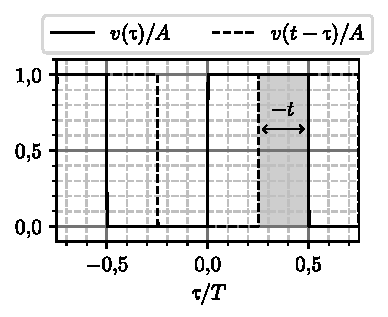
\includegraphics[page=1]{fig/cconv.pdf}    
        \caption{Случај за $t<0$.}
    \end{subfigure}
    %
    \begin{subfigure}[c]{0.49\textwidth}
        \centering
        \includegraphics[page=2]{fig/cconv.pdf}    
        \caption*{Случај за $t<0$.}
    \end{subfigure}
    \caption{Уз израчунавање дефиниционог интеграла.}
    \label{fig:\ID.int}
\end{figure}

Због транслаторне симетрије граница интеграције, период сигнала $v\circledast v$ је такође $T$.
Аналитичко решење датог интеграла је сложено због компликованих преклапања праоугаоних импулса који 
постоје у сигналу, па га је из тог разлога једноставније дискутовати графички. Израз 
$v(t-\uptau)$, посматрајући $\uptau$ на апсциси, представља сигнал пресликан око ординате па затим 
закашњен за $t$. Разликујемо два случаја, када је $t>0$ и када је $t<0$, као што је приказано 
на слици \ref{fig:\ID.int}, према чему је 
\begin{equation}
    v \circledast v = \begin{cases}
        A^2 t, & t > 0 \\
        -A^2 t & t < 0
    \end{cases}.
\end{equation}
График добијеног сигнала представљен је на слици \ref{fig:\ID.kk}. На основу добијене слике може се закључити да тај 
резултат представља поворку троугаоних импулса ширине $T$ и висине $A^2/2$, што се може записати скалирањем 
аргумента и множењем константом као 
\begin{equation}
    v \circledast v = 
    \dfrac{A^2 T}{2}
    \sum_{k = -\infty}^{\infty}  
    {\rm tri}\left( 
    \dfrac{2(t - kT)}{T} - 1
    \right).    
\end{equation}

\begin{figure}[ht!]
    \centering
    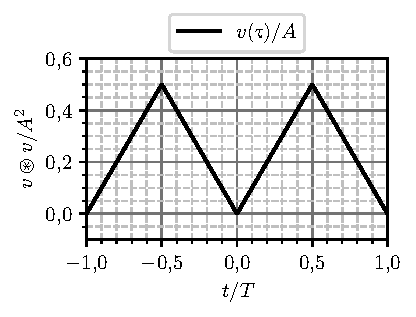
\includegraphics{fig/cconv_r3.pdf}
    \caption{Уз резултат.}
    \label{fig:\ID.kk}
\end{figure}

